\documentclass[12pt,letterpaper]{article}
\author{}
\usepackage[utf8]{inputenc}
\usepackage[spanish]{babel}
\usepackage{amsmath}
\usepackage{amsfonts}
\usepackage{graphicx}
\usepackage{geometry}
\usepackage{float}
\usepackage{caption}
\usepackage{csquotes}
\usepackage[style=apa, backend=biber]{biblatex}
\addbibresource{resources/referencias.bib}
\geometry{top=2.5cm, bottom=2.5cm, left=3cm, right=3cm}
\renewcommand{\baselinestretch}{1.2}

\title{Proyecto de Investigación \\ \textbf{Implementación Simplificada de PageRank utilizando Álgebra Lineal}}

\begin{document}

\maketitle
\newpage

% !TeX root = ../main.tex

\section{Marco Teórico}

\subsection{Grafos y representación matricial}
Los grafos son estructuras fundamentales en las matemáticas y la computación, y se utilizan para modelar las relaciones o conexiones entre distintos objetos. Este modelo tiene dos elementos principales:
\begin{itemize}
    \item \textbf{Vértices (o nodos $V$):} En nuestro caso, representan las páginas web individuales.
    \item \textbf{Aristas (o enlaces $E$):} En nuestro caso, serían las conexiones o hipervínculos que unen los nodos.
\end{itemize}

Hice un ejemplo sobre un canal de YouTube en el que existen 4 otras páginas conectadas: el Twitter del canal, el Facebook, un Fan Blog y un post de noticias.

\subsection{Matrices de transición probabilística}
Usando los nodos y enlaces, crearemos una matriz que utilizaremos para ejecutar el algoritmo PageRank. La matriz inicial se llama \textbf{matriz de adyacencia}.

Nuestra matriz se representa con las filas (origen) y sus columnas (destino). Se agrega un 1 en la intersección de la fila $i$ y la columna $j$ si entre las dos páginas hay un hipervínculo directo, y un 0 si no están conectadas.

Para añadir probabilidades, utilizamos las \textbf{Cadenas de Markov}. Una Cadena de Markov es un modelo que asume que la probabilidad de navegar hacia una nueva página depende únicamente de los hipervínculos disponibles en la página actual, sin importar de dónde venga el usuario.

Básicamente, para construir la matriz de transición probabilística, se toma la matriz de adyacencia que ya tenemos y se divide cada enlace por la cantidad total de hipervínculos salientes que hay en esa página. Al aplicar esto, obtendremos fracciones que, al sumarlas por fila, siempre nos darán 1 (el 100\% de probabilidad).

\subsection{Autovalores y autovectores}
Podemos seguir iterando el sistema (multiplicando las matrices) para conseguir un resultado más preciso y estabilizarlo. Al momento en donde los números ya no cambian y encuentran su equilibrio definitivo se le llama \textbf{convergencia}.

Cuando el proceso iterativo alcanza este punto de equilibrio, el momento en que vuelvas a multiplicar el vector por la matriz de transición una vez más y el resultado te dé exactamente el mismo vector original, es cuando pasamos a llamar a ese vector el \textbf{Autovector} del sistema (estado estacionario). Este autovector dominante, que está asociado al autovalor igual a 1, garantiza que exista un único estado estacionario. Los valores matemáticos dentro de este autovector representan el ranking final de PageRank, lo que define directamente la \textbf{importancia relativa de los nodos} dentro de la red.

% !TeX root = ../main.tex

\section{Representación de Redes}

\subsection{Construcción del grafo}
El diagrama de nuestro ejemplo se ve así:

\begin{figure}[H]
    \centering
    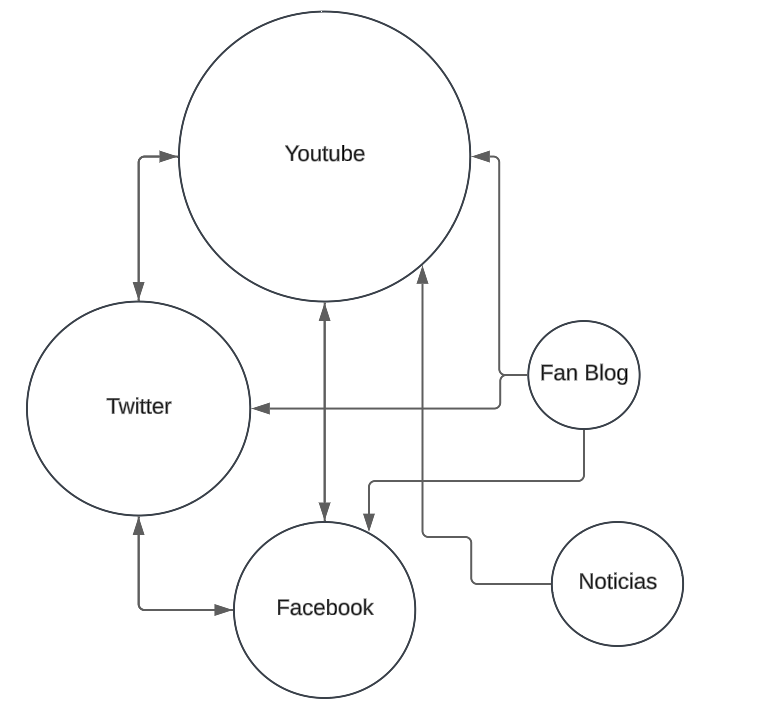
\includegraphics[width=0.7\textwidth]{resources/diagrama1.png}
    \caption{Visualización del grafo dirigido del ecosistema del canal.}
\end{figure}

En el ejemplo, las conexiones fluyen de la siguiente manera:
\begin{itemize}
    \item El canal de YouTube dirige a su Twitter y Facebook. [cite: 15]
    \item El Twitter enlaza hacia el canal de YouTube y el Facebook. [cite: 16]
    \item El Facebook enlaza al Twitter y al canal de YouTube. [cite: 17]
    \item El Fan Blog enlaza al Facebook, al canal de YouTube y al Twitter. [cite: 18]
    \item El post de noticias enlaza únicamente al canal de YouTube. [cite: 19]
\end{itemize}

\subsection{Representación matricial}
Usando este diagrama de conexiones, nos daría la siguiente matriz de adyacencia:
(Recordemos que la primera fila es Youtube, la segunda Twitter, la tercera Facebook, cuarta Fan Blog, quinta Noticias)

\begin{equation}
    A = \begin{pmatrix}
    0 & 1 & 1 & 0 & 0 \\
    1 & 0 & 1 & 0 & 0 \\
    1 & 1 & 0 & 0 & 0 \\
    1 & 1 & 1 & 0 & 0 \\
    1 & 0 & 0 & 0 & 0
    \end{pmatrix} [cite: 20]
\end{equation}

Le aplicamos la lógica de las cadenas de Markov y vemos cómo las fracciones dependen de la cantidad total de hipervínculos de salida en cada página, dándonos esta matriz de transición ($P$):

\begin{equation}
    P = \begin{pmatrix}
    0 & 1/2 & 1/2 & 0 & 0 \\
    1/2 & 0 & 1/2 & 0 & 0 \\
    1/2 & 1/2 & 0 & 0 & 0 \\
    1/3 & 1/3 & 1/3 & 0 & 0 \\
    1 & 0 & 0 & 0 & 0
    \end{pmatrix} [cite: 21]
\end{equation}

\subsection{Iteraciones del algoritmo}
Tomamos nuevamente el ejemplo del diagrama de antes y hacemos las iteraciones. [cite: 22] Para entender de dónde salen los valores de los vectores, realizamos una operación matemática llamada multiplicación de un vector por una matriz. [cite: 23] Para calcular el nuevo puntaje de una página, multiplicamos el vector de probabilidades actual por la columna correspondiente a esa página en la matriz de transición. [cite: 24]

\textbf{1. El punto de partida ($v_0$):}
Iniciamos con un vector donde todos los nodos tienen la misma probabilidad inicial ($1/5$). [cite: 25]
\begin{equation}
    v_0 = \begin{pmatrix} 1/5 & 1/5 & 1/5 & 1/5 & 1/5 \end{pmatrix} [cite: 26]
\end{equation}

\textbf{2. La multiplicación (Producto punto):}
Multiplicamos cada valor de $v_0$ por su valor correspondiente en la primera columna de la matriz $P$ (que contiene las probabilidades de que el resto de las páginas enlacen a YouTube) y sumamos los resultados:
\begin{equation}
    v_1(\text{YouTube}) = \left(\frac{1}{5} \cdot 0\right) + \left(\frac{1}{5} \cdot \frac{1}{2}\right) + \left(\frac{1}{5} \cdot \frac{1}{2}\right) + \left(\frac{1}{5} \cdot \frac{1}{3}\right) + \left(\frac{1}{5} \cdot 1\right) [cite: 27]
\end{equation}

\textbf{3. La suma de fracciones:}
\begin{equation}
    v_1(\text{YouTube}) = 0 + \frac{1}{10} + \frac{1}{10} + \frac{1}{15} + \frac{1}{5}
\end{equation}

Buscando el denominador común (30):
\begin{equation}
    v_1(\text{YouTube}) = 0 + \frac{3}{30} + \frac{3}{30} + \frac{2}{30} + \frac{6}{30} = \frac{14}{30}
\end{equation}

Simplificando la fracción, obtenemos el valor exacto para YouTube en la primera iteración:
\begin{equation}
    v_1(\text{YouTube}) = \frac{7}{15}
\end{equation}

Aplicando este mismo procedimiento para cada columna y repitiéndolo en cada paso, vemos cómo los vectores completos evolucionan en nuestras 3 iteraciones:

\textbf{Iteración 1 ($v_1 = v_0 \cdot P$):}
\begin{equation*}
    v_1 = \begin{pmatrix} \frac{1}{5} & \frac{1}{5} & \frac{1}{5} & \frac{1}{5} & \frac{1}{5} \end{pmatrix} \cdot P = \begin{pmatrix} \frac{7}{15} & \frac{4}{15} & \frac{4}{15} & 0 & 0 \end{pmatrix} [cite: 28]
\end{equation*}

\textbf{Iteración 2 ($v_2 = v_1 \cdot P$):}
\begin{equation*}
    v_2 = \begin{pmatrix} \frac{7}{15} & \frac{4}{15} & \frac{4}{15} & 0 & 0 \end{pmatrix} \cdot P = \begin{pmatrix} \frac{8}{30} & \frac{11}{30} & \frac{11}{30} & 0 & 0 \end{pmatrix}
\end{equation*}

\textbf{Iteración 3 ($v_3 = v_2 \cdot P$):}
\begin{equation*}
    v_3 = \begin{pmatrix} \frac{8}{30} & \frac{11}{30} & \frac{11}{30} & 0 & 0 \end{pmatrix} \cdot P = \begin{pmatrix} \frac{22}{60} & \frac{19}{60} & \frac{19}{60} & 0 & 0 \end{pmatrix}
\end{equation*}

\subsection{Interpretación del ranking obtenido}
Como vemos, el número más grande dentro de los vectores finales es de la página de YouTube ($\frac{22}{60}$). [cite: 29] Esto significa que la página con más relevancia (autoridad) es YouTube, y esto se debe a que es la página que recibe más enlaces importantes hacia ella. [cite: 30] También podemos ver que el Fan Blog y la página de Noticias son equivalentes a 0 en las iteraciones. [cite: 31] Esto se debe a que ninguna de las páginas de la red enlaza hacia ellos, por lo que el "navegante aleatorio" nunca los visita. [cite: 32]
% !TeX root = ../main.tex

\section{Implementación computacional}
% !TeX root = ../main.tex

\section{Reflexión y Conclusiones}
El modelamiento de sistemas computacionales e infraestructuras a través de la teoría de grafos y el álgebra lineal permite abstraer la complejidad topológica hacia representaciones matriciales (como la matriz de adyacencia o transición). 
Esta cuantificación matemática habilita la aplicación de métodos numéricos para predecir comportamientos, identificar vulnerabilidades y priorizar información. El algoritmo PageRank constituye uno de los ejemplos más significativos de esta 
transición entre la teoría algebraica pura y la ingeniería de software aplicada.

\subsection{Ventajas y limitaciones del algoritmo PageRank}
El análisis operativo del algoritmo revela métricas de rendimiento y vulnerabilidades teóricas que deben ser consideradas en su implementación: 

\begin{itemize}
    \item \textbf{Escalabilidad y complejidad computacional:} El cálculo directo de autovalores para una matriz presenta una complejidad temporal polinomial de $O(N^3)$, resultando computacionalmente intratable para un grafo 
    web con miles de millones de nodos. Sin embargo, la gran ventaja de PageRank radica en la utilización del método iterativo de las potencias operando sobre la matriz de adyacencia dispersa (y aplicando el factor de amortiguamiento 
    como un término constante). Al almacenar únicamente los coeficientes no nulos (los enlaces existentes), la complejidad computacional se reduce significativamente a $O(k \cdot E)$, donde $k$ es el número de iteraciones y $E$ es el número de aristas. \parencite{tigergraph}
    \item \textbf{Manipulación de enlaces:} Dado que la autoridad se fundamenta en la suma ponderada de enlaces entrantes, el sistema es susceptible a vulneraciones topológicas conocidas como Link Farming (granjas de enlaces). 
    Esta manipulación consiste en la creación deliberada de redes artificiales de nodos (sitios web falsos) altamente interconectados entre sí, con el único propósito de concentrar probabilidad y dirigirla hacia un nodo objetivo, 
    inflando artificialmente el valor numérico de su autovector principal y alterando la legitimidad del ranking. \parencite{needmylink2025}
\end{itemize}

\subsection{PageRank en la actualidad}
La aplicación de este algoritmo no se limita al motor de búsqueda de Google. Aunque fue diseñado originalmente con ese propósito, matemáticamente PageRank es un algoritmo genérico de centralidad basado en autovectores, 
el cual permite su extrapolación a múltiples áreas científicas e industriales:

\begin{itemize}
    \item \textbf{Redes sociales y análisis de influencia:} Redes sociales como la conocida X (anteriormente Twitter) aplican variantes estocásticas como Personalized PageRank para modelar la propagación de información. 
    En este contexto, los nodos representan usuarios y las aristas dirigidas denotan relaciones de seguimiento o interacción. El estado estacionario permite identificar a los hubs de información y optimizar los sistemas 
    de recomendación (algoritmos que recomiendan a quien seguir). \parencite{tao2021}
    \item \textbf{Procesamiento de Lenguaje Natural (PLN):} Algoritmos modernos como TextRank utilizan la lógica algebraica de PageRank para tareas de PLN como resumen y extracción de palabras clave. En este modelo, 
    las palabras u oraciones se definen como nodos, y la similitud semántica actúa como el enlace ponderado, calculando así el texto más representativo del documento. \parencite{yassine2025}
    \item \textbf{Sistemas de Recomendación y E-commerce:} Mediante la construcción de grafos bipartitos que modelan las interacciones entre usuarios y catálogos de productos, la aplicación del método de la potencia 
    sobre sus matrices de transición permite obtener un vector de probabilidad estacionario que infiere preferencias latentes. La propagación del peso algebraico a través de estos enlaces permite sugerir artículos a 
    consumidores basándose en la concentración de probabilidad generada por usuarios con patrones de consumo homólogos. \parencite{lorenzo2022}
\end{itemize}

\printbibliography
\end{document}